% flashcards-title: Matching leftward movements
% flashcards-desc: Two parallel number lines both move three units left from two to negative one, labeled subtract three and add negative three.
\documentclass[dvisvgm,tikz,border=8pt]{standalone}
\usetikzlibrary{arrows.meta,patterns}

\definecolor{qraNavy}{HTML}{17324D}
\definecolor{qraBlue}{HTML}{2B6CB0}
\definecolor{qraGold}{HTML}{B7791F}
\definecolor{qraPale}{HTML}{EAF2F8}
\definecolor{qraGray}{HTML}{5C6773}

\tikzset{
  qra axis/.style={draw=qraNavy, line width=1.2pt},
  qra tick/.style={draw=qraNavy, line width=1pt},
  qra guide/.style={draw=qraGray, densely dashed, line width=0.8pt},
  qra counter/.style={circle, draw=qraNavy, fill=qraPale, line width=0.9pt, minimum size=7mm, inner sep=0pt},
  qra label/.style={font=\sffamily\bfseries, text=qraNavy},
  qra small label/.style={font=\sffamily, text=qraNavy},
}

\begin{document}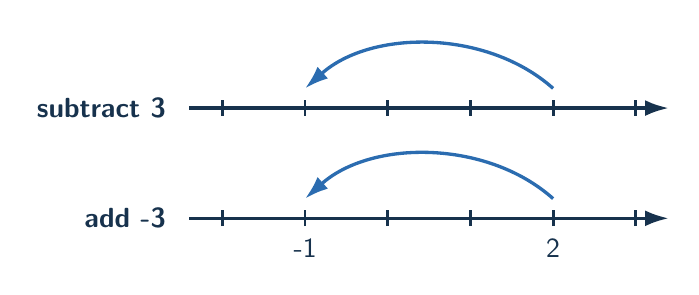
\begin{tikzpicture}[x=1.05cm,y=1cm]
\foreach \y/\lab in {1.4/{subtract 3},0/{add -3}}{\draw[qra axis,-{Latex[length=3mm,width=2mm]}](-2.4,\y)--(3.4,\y);\foreach \x in {-2,...,3}{\draw[qra tick](\x,\y-.1)--(\x,\y+.1);}\draw[qraBlue,line width=1.2pt,-{Latex[length=3mm,width=2mm]}](2,\y+.25)..controls(1.2,\y+1)and(-.2,\y+1)..(-1,\y+.25);\node[qra label,left=5pt]at(-2.4,\y){\lab};}
\node[qra small label,below=4pt]at(-1,0){-1};\node[qra small label,below=4pt]at(2,0){2};
\end{tikzpicture}\end{document}
